% !TEX root=ricardo_draft.tex
% In this section we evaluate our framework for modeling fairness.

%%%% TODO!!! ADD COMMENT THAT WE NEED Y TO LEARN THE CAUSAL MODEL!!!!!

\section*{S1 Population Level vs Individual Level Causal Effects}
\label{sec:individual}

As discussed in Section~\ref{sec:count_fair}, counterfactual fairness
is an individual-level definition. This is fundamentally different
from comparing different units that happen to share the same
“treatment” $A = a$ and coincide on the values of $X$. To see in
detail what this means, consider the following thought experiment.

Let us assess the causal effect of $A$ on $\hat Y$ by controlling
$A$ at two levels, $a$ and $a'$. In Pearl's notation, where ``$do(A = a)$''
expresses an intervention on $A$ at level $a$, we have that
\begin{equation}
\label{eq:ace}
\mathbb{E}[\hat Y\ |\ do(A = a), X = x] - \mathbb{E}[\hat Y\ |\ do(A = a'), X = x],
\end{equation}
is a measure of causal effect, sometimes called the average causal
effect (ACE). It expresses the change that is expected when we
intervene on $A$ while observing the attribute set $X = x$, under two
levels of treatment. If this effect is non-zero, $A$ is considered to
be a cause of $\hat Y$.

This raises a subtlety that needs to be addressed: in general, this
effect will be non-zero {\it even if $\hat Y$ is counterfactually
  fair}. This may sound counter-intuitive: protected attributes such
as race and gender are causes of our counterfactually fair decisions.

In fact, this is not a contradiction, as the ACE in Equation
(\ref{eq:ace}) is different from counterfactual effects. The ACE
contrasts two independent exchangeable units of the population, and it
is a perfectly valid way of performing decision analysis. However, the
value of $X = x$ is affected by different background variables
corresponding to different individuals. That is, the causal effect
(\ref{eq:ace}) contrasts two units that receive different treatments
but which happen to coincide on $X = x$. To give a synthetic example,
imagine the simple structural equation
\[
X = A + U.
\]

The ACE quantifies what happens among people with $U = x -
a$ against people with $U' = x - a'$. If, for instance, $\hat Y =
\lambda U$ for $\lambda \neq 0$, then the effect \eqref{eq:ace}
is $\lambda(a - a') \neq 0$.

Contrary to that, the counterfactual difference is zero.
That is,
\[
\mathbb{E}[\hat Y_{A \leftarrow a}(U)\ |\ A = a, X = x] -
\mathbb{E}[\hat Y_{A \leftarrow a'}(U)\ |\ A = a, X = x] =
\lambda U - \lambda U = 0.
\]

In another perspective, we can interpret the above just as if we had
{\it measured} $U$ from the beginning rather than performing
abduction. We then generate $\hat Y$ from some $g(U)$, so $U$ is the
within-unit cause of $\hat Y$ and not $A$.

If $U$ cannot be deterministically derived from $\{A = a, X = x\}$,
the reasoning is similar. By abduction, the distribution of $U$ will
typically depend on $A$, and hence so will $\hat Y$ when marginalizing
over $U$. Again, this seems to disagree with the intuition that our
predictor should be not be caused by $A$. However, this once again is
a comparison {\it across individuals}, not within an individual. 

It is this balance among $(A, X, U)$ that explains, in the examples
of Section~\ref{sec:further_examples}, why some predictors are
counterfactually fair even though they are functions of the same
variables $\{A, X\}$ used by unfair predictors: such functions must
correspond to particular ways of balancing the observables that, by
way of the causal assumptions, cancel out the effect of $A$.

\noindent {\bf More on conditioning and alternative definitions.} As discussed in
Example 4.4.4 of \citet{pearl:16}, a different proposal for
assessing fairness can be defined via the following concept:
\begin{define}[Probability of sufficiency]
  We define the probability of event $\{ A = a \}$ being a
  \emph{sufficient cause} for our
  decision $\hat Y$, contrasted against $\{ A = a' \}$, as
\begin{align}
  P(\hat Y_{A \leftarrow a'\ }(U) \neq y\ |\ X = x, A = a, \hat Y = y).
\end{align}
\end{define}

We can then, for instance, claim that $\hat Y$ is a fair predictor if
this probability is below some pre-specified bound for all $(x, a,
a')$. The shortcomings of this definition come from its original
motivation: to {\it explain} the behavior of an {\it existing}
decision protocol, where $\hat Y$ is the current practice and which in a
unclear way is conflated with $Y$. The implication is that if $\hat Y$
is to be designed instead of being a natural measure of existing
behaviour, then we are using $\hat Y$ itself as evidence for the
background variables $U$. This does not make sense if $\hat Y$ is
yet to be designed by us. If $\hat Y$ is to be interpreted as $Y$, then this
does not provide a clear recipe on how to build $\hat Y$: while we can
use $Y$ to learn a causal model, we cannot use it to collect training
data evidence for $U$ {\it as the outcome $Y$ will not be available to
  us at prediction time}. For this reason, we claim that while
probability of sufficiency is useful as a way of assessing an existing
decision making process, it is not as natural as counterfactual
fairness in the context of machine learning.

\noindent {\bf Approximate fairness and model validation.} The notion
of probability of sufficiency raises the question on how to define
approximate, or high probability, counterfactual fairness. This is an
important question but for reasons of conciseness and focus we defer
it entirely to future work. Before defining an approximation, it is
important to first expose in detail what the exact definition is,
which is the goal of this paper.

We also do not address the validation of the causal assumptions used
by the input causal model of the {\sc FairLearning} algorithm in
Section \ref{sec:algorithm}. The reason is straightforward: this
validation is an entirely self-contained step of the implementation of
counterfactual fairness. An extensive literature already exists in
this topic which the practitioner can refer to (a classic account for
instance is \cite{bollen:93}), and which can be used as-is in our
context.

The experiments performed in Section \ref{sec:experiments} can be
criticized by the fact that they rely on a model that obeys our
assumptions, and ``obviously'' our approach should work better than
alternatives. This criticism is not warranted: in machine learning,
causal inference is typically assessed through simulations which
assume that the true model lies in the family covered by the
algorithm.  Algorithms, including {\sc FairLearning}, are justified in
the population sense. How different competitors behave with finite
sample sizes is the primary question to be studied in an empirical
study of a new concept, where we control for the correctness of the
assumptions. Although sensitivity analysis is important, there are
many degrees of freedom on how this can be done. Robustness issues are
better addressed by extensions focusing on approximate versions of 
counterfactual fairness. This will be covered in later work.

\section*{S2 Relation to Demographic Parity}
%
Consider the graph $A \rightarrow X \rightarrow Y$. In general, if
$\hat Y$ is a function of $X$ only, then $\hat Y$ need not obey
demographic parity, i.e.
\begin{align}
  P(\hat Y\ |\ A = a) \neq P(\hat Y\ |\ A = a'),\nonumber
\end{align}
\noindent where, since $\hat Y$ is a function of $X$, the
probabilities are obtained by marginalizing over $P(X\ |\ A = a)$ and
$P(X\ |\ A = a')$, respectively.

If we postulate a structural equation $X = \alpha A + e_X$, then given
$A$ and $X$ we can deduce $e_X$. If $\hat Y$ is a function of $e_X$
only and, by assumption, $e_X$ is marginally independent of $A$, then
$\hat Y$ is marginally independent of $A$: this follows the
interpretation given in the previous section, where we interpret $e_X$
as ``known'' despite being mathematically deduced from the
observation $(A = a, X = x)$. Therefore, the assumptions imply that
$\hat Y$ will satisfy demographic parity, and that can be falsified.
By way of contrast, if $e_X$ is not uniquely identifiable from the
structural equation and $(A, X)$, then the distribution of $\hat Y$
depends on the value of $A$ as we marginalize $e_X$, and demographic
parity will not follow. This leads to the following:
%
\begin{lem}
If all background variables $U' \subseteq U$ in the definition of
$\hat Y$ are determined from $A$ and $X$,
and all observable variables in the definition of $\hat Y$ are
independent of $A$ given $U'$, then $\hat Y$ satisfies demographic
parity.
% If the conditions fail, then $\hat Y$ will not satisfy demographic parity in general. 
\end{lem}
Thus, counterfactual fairness can be thought of as a counterfactual
analog of demographic parity, as present in the Red Car example further discussed
in the next section.

\section*{S3 Examples Revisited}

In Section \ref{sec:further_examples}, we discussed two examples. We
reintroduce them here briefly, add a third example, and explain some
consequences of their causal structure to the design of
counterfactually fair predictors.

\paragraph{Scenario 1: The Red Car Revisited.}
In that scenario, the structure $A \rightarrow X \leftarrow U
\rightarrow Y$ implies that $\hat Y$ should not use either $X$ or
$A$. On the other hand, it is acceptable to use $U$.  It is
interesting to realize, however, that since $U$ is related to $A$ and
$X$, there will be some association between $Y$ and $\{A, X\}$ as
discussed in Section S1. In particular, if the structural equation for
$X$ is linear, then $U$ is a linear function of $A$ and $X$, and as
such $\hat Y$ will also be a function of both $A$ and $X$. This is not
a problem, as it is still the case that the model implies that this is
merely a functional dependence that disappears by conditioning on a
postulated latent attribute $U$. Surprisingly, we must make $\hat Y$ a
indirect function of $A$ if we want a counterfactually fair predictor,
as shown in the following Lemma.

  %
\begin{lem}
Consider a linear model with the structure in
Figure~\ref{figure.simple_models}(d).  Fitting a linear predictor to
$X$ \emph{only} is not counterfactually fair, while the same algorithm
will produce a fair predictor using \emph{both} $A$ and $X$.
\end{lem}
%
\begin{proof}
As in the definition, we will consider the population case, where the
joint distribution is known. Consider the case where the equations
described by the model in Figure~\ref{figure.simple_models}(d)
are deterministic and linear:
\begin{align}
X = \alpha A + \beta U, \;\;\;\; Y = \gamma U. \nonumber
\end{align}
Denote the variance of $U$ as $v_U$, the variance of $A$ as $v_A$, and
assume all coefficients are non-zero. The predictor $\hat Y(X)$
defined by least-squares regression of $Y$ on \emph{only} $X$ is given
by $\hat Y(X) \equiv \lambda X$, where $\lambda = Cov(X, Y) / Var(X)
\!=\! \beta\gamma v_U / (\alpha^2 v_A + \beta^2 v_U) \neq 0$. This 
predictor follows the concept of fairness through unawareness.

We can test whether a predictor $\hat{Y}$ is counterfactually fair
by using the procedure described in Section~\ref{subsec:cmc}:
%\begin{itemize}
{\em (i)} Compute $U$ given observations of $X,Y,A$; %, by solving for $U$.
{\em (ii)} Substitute the equations involving $A$ with an interventional value $a'$; 
% (i.e., this says: `what happens if the race of an individual were changed')
{\em (iii)} Compute the variables $X,Y$ with the interventional value
$a'$. It is clear here that $\hat Y_a(U) \!=\! \lambda(\alpha a +
\beta U) \neq \hat Y_{a'}(U)$. This predictor is not counterfactually
fair. Thus, in this case fairness through unawareness actually
perpetuates unfairness.

Consider instead doing least-squares regression of $Y$ on $X$
\emph{and} $A$. Note that $\hat Y(X,A) \equiv \lambda_X X + \lambda_A
A$ where $\lambda_X,\lambda_A$ can be derived as follows:
\begin{align}
\begin{pmatrix}
\lambda_X \\
\lambda_A
\end{pmatrix} &=
\begin{pmatrix}
Var(X) & Cov(A,X) \\
Cov(X,A) & Var(A)
\end{pmatrix}^{-1}
\begin{pmatrix}
Cov(X,Y) \\
Cov(A,Y)
\end{pmatrix} \nonumber \\
&=
%\frac{1}{(\alpha^2 v_A + \beta^2 v_U)v_A - \alpha^2 v_A^2}
\frac{1}{\beta^2 v_U v_A}
\begin{pmatrix}
v_A & -\alpha v_A \\
-\alpha v_A & \alpha^2 v_A + \beta^2 v_U
\end{pmatrix}
\begin{pmatrix}
\beta \gamma v_U \\
0
\end{pmatrix} \nonumber \\
&=
\begin{pmatrix}
\frac{\gamma}{\beta} \\
\frac{-\alpha\gamma}{\beta}
%(-\alpha\gamma) / \beta
\end{pmatrix}
\end{align}
Now imagine we have observed $A\!=\!a$. This implies that $X = \alpha
a + \beta U$ and our predictor is $\hat Y(X,a) =
\frac{\gamma}{\beta}(\alpha a + \beta U) + \frac{-\alpha\gamma}{\beta}
a = \gamma U$. Thus, if we substitute $a$ with a counterfactual $a'$
(the action step described in Section~\ref{subsec:cmc}) the predictor
$\hat Y(X,A)$ is unchanged. This is because our predictor is
constructed in such a way that any change in $X$ caused by a change in
$A$ is cancelled out by the $\lambda_A$. Thus this predictor is
counterfactually fair.
% This is known to be equivalent to first getting the residuals $R_X$ of $X$ regressed on $A$
% and regressing $Y$ on $R_X$ and $A$. Notice that $R_X \!=\! U$, and $A$ is independent of $U$
% and $Y$. Hence, $\hat Y$ will be the least squares regression of
% $Y$ on $U$, resulting on $\hat Y \!=\! \gamma U$, which is counterfactually fair.
\end{proof}

Note that if Figure~\ref{figure.simple_models}(d) is the
true model for the real world then $\hat Y(X,A)$ will also satisfy
demographic parity and equality of opportunity as $\hat Y$ will be
unaffected by $A$. 

The above lemma holds in a more general case for the structure given
in Figure~\ref{figure.simple_models}(d): any non-constant
estimator that depends only on $X$ is not counterfactually fair as
changing $A$ always alters $X$.
%We also point out that the method
%used in the proof is a special case of a general method to building a
%predictor based on information deduced about $U$ that will be
%described in the next section.

\paragraph{Scenario 2: High Crime Regions Revisited.}

The causal structure differs from the previous example by the extra
edge $X \rightarrow Y$. For illustration purposes, assume again that
the model is linear. Unlike the previous case, a predictor $\hat Y$
trained using $X$ and $A$ is not counterfactually fair. The only
change from Scenario 1 is that now $Y$ depends on $X$ as follows: $Y
\!=\! \gamma U + \theta X$. Now if we solve for $\lambda_X,\lambda_A$
it can be shown that $\hat Y(X,a) \!=\! (\gamma - \frac{\alpha^2
  \theta v_A}{\beta v_U})U + \alpha \theta a$. As this predictor
depends on the values of $A$ that are not explained by $U$, then
$\hat Y(X,a) \!\neq\! \hat Y(X,a')$ and thus $\hat Y(X,A)$ is not
counterfactually fair.

The following extra example complements the previous two examples.

\paragraph{Scenario 3: University Success.}
A university wants to know if students will be successful
post-graduation $Y$. They have information such as: grade point
average (GPA), advanced placement (AP) exams results, and other
academic features $X$. The university believes however, that an
individual's gender $A$ may influence these features and their
post-graduation success $Y$ due to social discrimination. They also
believe that independently, an individual's latent talent $U$ causes
$X$ and $Y$. The structure is similar to
Figure~\ref{figure.simple_models}(d), with the extra
edge $A \rightarrow Y$. We can again ask, is the predictor $\hat
Y(X,A)$ counterfactually fair? In this case, the different between
this and Scenario 1 is that $Y$ is a function of $U$ and $A$ as
follows: $Y \!=\! \gamma U + \eta A$. We can again solve for
$\lambda_X,\lambda_A$ and show that $\hat Y(X,a) \!=\! (\gamma -
\frac{\alpha \eta v_A}{\beta v_U})U + \eta a$. Again $\hat Y(X,A)$ is
a function of $A$ not explained by $U$, so it cannot be counterfactually fair.

% We propose to model the law school data as shown in
% Figure~\ref{figure.law_school}. We suspect that variables race and sex
% affect student performance (e.g. GPA, LSAT, and FYA) due to factors
% such as cultural norms, which assume that individuals of a certain
% race or sex are `better suited' to be lawyers. Such beliefs could
% adversely impact students who do not fit these norms. Instead we would
% like to model the latent \emph{knowledge} (K) of a student, which also
% impacts these features. 
% We can then construct a predictor that
% predicts FYA fairly using knowledge. It is easy to show that such a predictor
% is counterfactually fair, whereas a predictor that uses features GPA and
% LSAT is not (in this case even including race and sex as
% features cannot correct this, as can be done in the linear case). The
% causal 
 %; %3. \textbf{Variational Fair Autoencoder (VFAE)} \cite{louizos2015variational}, a recent approach that works to learn a fair representation of the original data.
% compute counterfactuals for both race and sex

% \begin{table}[t]
% \vspace{-2ex}
% \caption{}
% \vspace{-3ex}
% \label{table.pred_law}
% \begin{center}
% \resizebox{\columnwidth}{!}
% {
% \begin{sc}
% \footnotesize
% \begin{tabular}{c|c|c|c}
% \hline
% %\multicolumn{5}{c}{\textbf{Lower Bounds}}\\
% \hline
% & full & unaware  & fair l2 & fair l3 \\
% \hline
% RMSE & 0.873 & 0.894 & 0.929 & 0.918 \\ \hline
% \end{tabular}
% \end{sc}
% }
% \end{center}
% \vspace{-4ex}
% \end{table}
%
%{lr@{$\pm$}lr@{$\pm$}lr@{$\pm$}l}

\section*{S4 Case Study: Criminality vs. Perceived Criminality}
\label{sec:true-vs.-perceived}

We test our approach on a problem of \emph{separating actual and
  perceived criminality in police stops}. For this problem, we
construct a causal model, and make explicit how unfairness may affect
observed and unobserved variables in the world. Given the model we
derive counterfactually fair predictors, and predict latent variables
such as a person's `criminality' (which may be useful for predicting
crime) as well as their `perceived criminality' (which may be due to
prejudices based on appearance). Finally we judge how well our
counterfactually fair `criminality' score satisfies demographic
parity.

\begin{figure*}[!t]
\begin{center}
\centerline{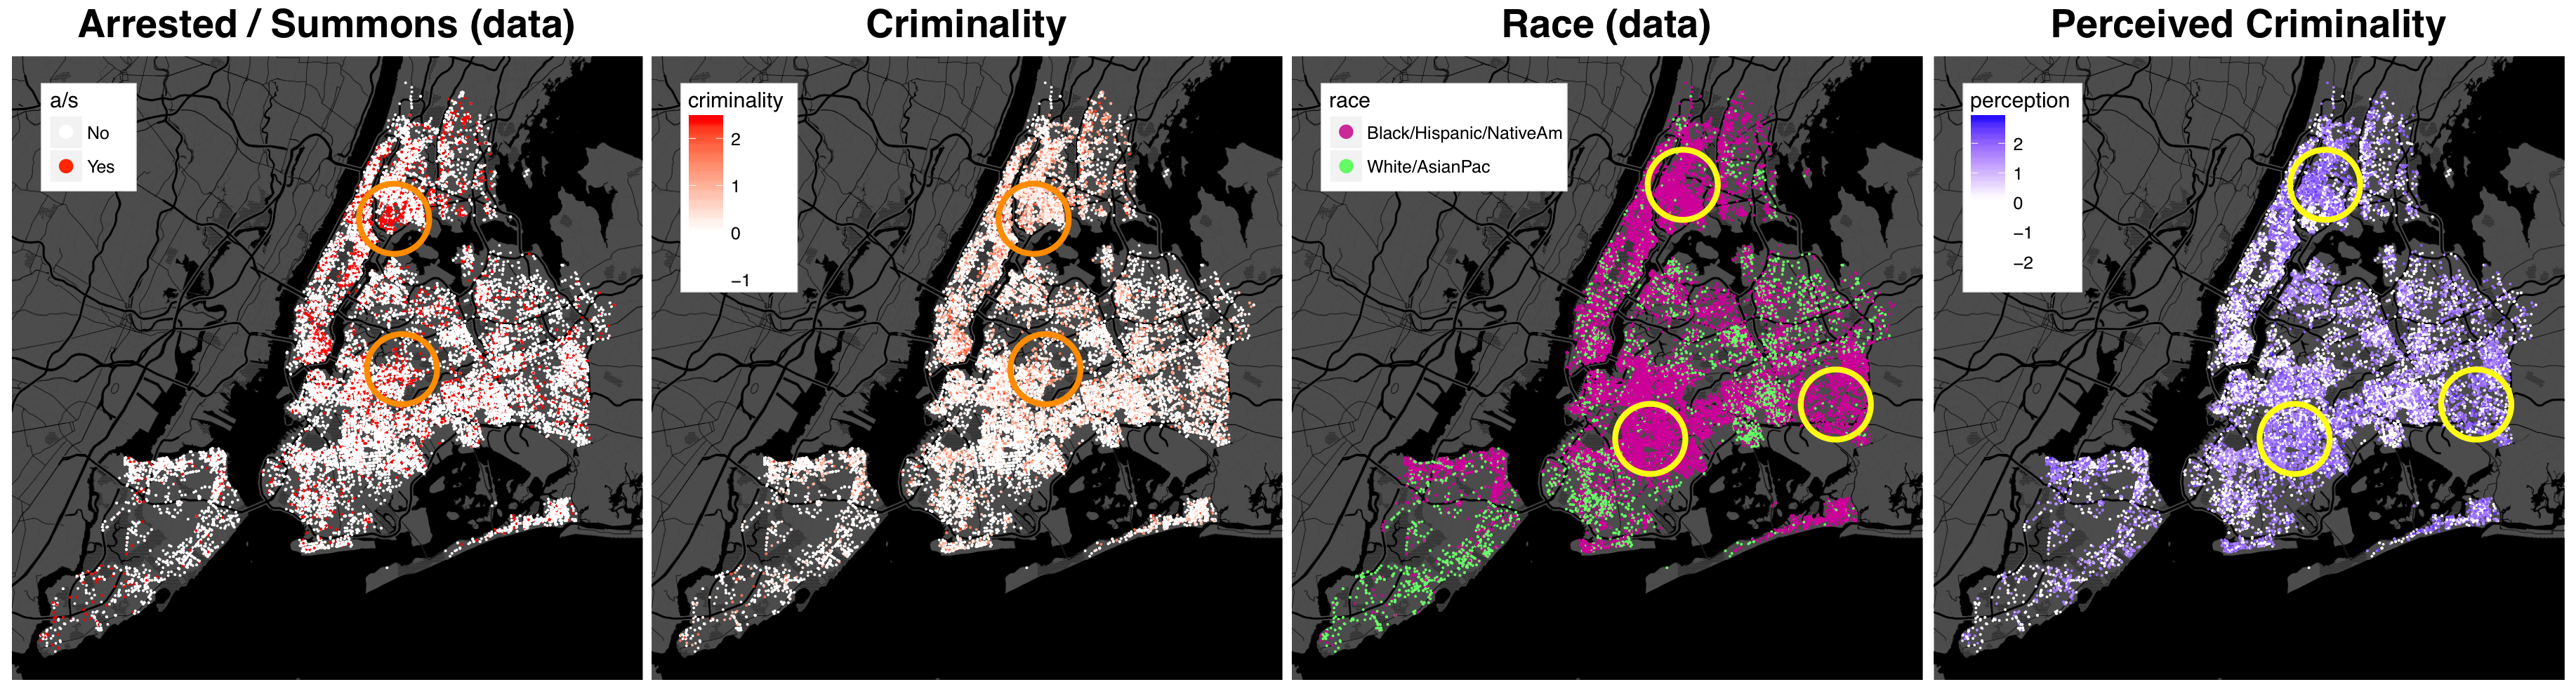
\includegraphics[width=\textwidth]{stop_and_frisk_graphs.png}}
\caption{Understanding criminality. The above maps show the
  decomposition of stop and search data in New York into factors based
  on perceived criminality (a race dependent variable) and latent
  criminality (a race neutral measure). See
  section~\ref{sec:true-vs.-perceived}.  \label{figure.criminality}\vspace{-7ex}}
\end{center}
\end{figure*}

Since 2002, the New York Police Department (NYPD) has recorded
information about every time a police officer has stopped someone. The
officer records information such as if the person was searched or
frisked, % if a weapon was found, their appearance, whether an arrest
was made or a summons issued, % if force was used, etc. We consider
the data collected on males stopped during 2014 which constitutes
38,609 records. % We limit our analysis to looking at just males
stopped as this accounts for more than $90\%$ of the data.  We fit a
model which decomposes these records into two latent factors, one
which depends on the race and appearance of the individual being
stopped, labeled \emph{Perceived Criminality}, and one which does not,
labeled \emph{Criminality}, and which could be used as a basis for
counterfactually fair decisions. The full details of this experiment,
including the DAG, are given in the supplementary materials. We now
describe a spatial analysis of the estimated latent factors.

\paragraph{Visualization on a map of New York City.}
Each of the stops can be mapped to longitude and latitude points for
where the stop
occurred\footnote{https://github.com/stablemarkets/StopAndFrisk}. Thus
we can visualize \emph{Criminality} and \emph{Perception} alongside
\emph{Race} and the combination of \emph{Arrest} and \emph{Summons},
shown in Figure~\ref{figure.criminality}.  Criminality seems to be a
continuous approximation of arrest and summons as both plots show red
in similar areas. However, the plots show that certain areas, while
having a lot of arrests have low criminality scores such as south
Bronx and west Queens (circled in orange). We can also compare the
perceived criminality with a plot of race, where we have divided the
races into Group A: black, black Hispanic, Hispanic, and Native
American (shown in purple); and Group B: white and Asian/Pacific
Islander (shown in green). Group A are all races that have positive
weights on the connection from \emph{Race} to \emph{Perception} in the
fitted model, while Group B all have negative weights. Thus being in
Group A leads one to have a higher perceived criminality than being in
Group B. This can be seen in the right-most plot of
Figure~\ref{figure.criminality}. Certain areas of town such as central
Brooklyn, central Bronx, and southern Queens have very high
criminality and almost all stops are by members of Group A (circled in
yellow).




%\subsection{Model criticism}
%%% Local Variables:
%%% mode: latex
%%% TeX-master: "ricardo_draft"
%%% End:
